\documentclass[aspectratio=169]{beamer}

\usepackage{tikzlings}

\setbeamertemplate{navigation symbols}{}
\setbeamertemplate{background canvas}{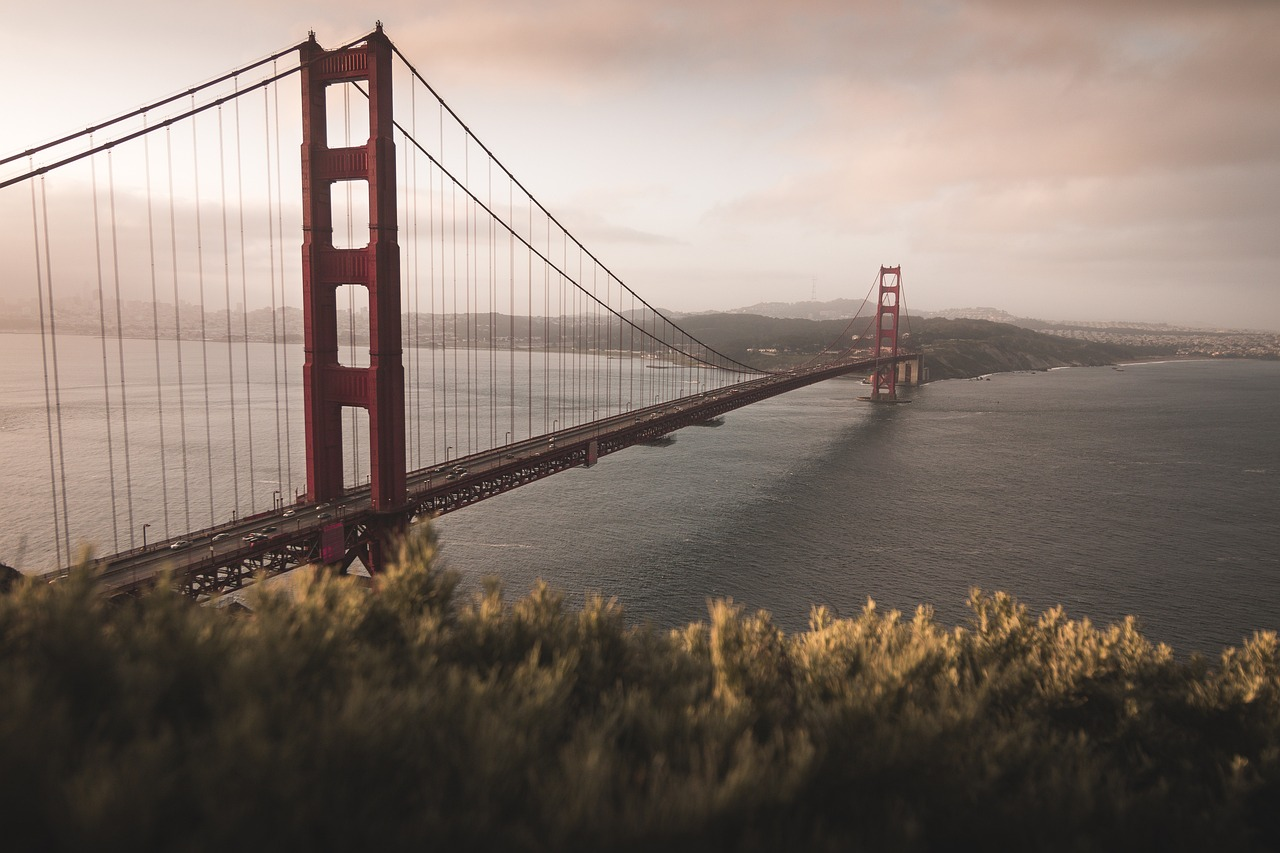
\includegraphics[width=\paperwidth]{golden-gate-bridge-4271364_1280}}
\graphicspath{{include/}}

% trick taken from https://topanswers.xyz/tex?q=1989
\tikzset{
    use page relative coordinates/.style={
        shift={(current page.south west)},
        x={(current page.south east)},
        y={(current page.north west)}
    },
}

\begin{document}

\begin{frame}
  \begin{tikzpicture}[remember picture, overlay,use page relative coordinates]

    \node[anchor=south,rotate=-5*sin(\insertoverlaynumber*3)] at (0.25,0.1) {
\includegraphics[height=3.8cm]{FP3}};
    \node[anchor=south,xscale=-1,rotate=5*sin(\insertoverlaynumber*3)] at (0.48,0.05) {
\includegraphics[height=4cm]{FP1}};
    \node[anchor=south,rotate=-5*sin(\insertoverlaynumber*3)] at (0.78,0.1) {
\includegraphics[height=4cm]{FP2}};

    % credit for background image
    \node[white,text width=.7\paperwidth,font=\tiny,align=center] at ([yshift=0.35cm]current page.south) {Image by @crispy-fotografie (\url{https://pixabay.com/de/photos/golden-gate-bridge-san-francisco-4271364/})};

  \end{tikzpicture}
  \pause[600]
\end{frame}

\end{document}